\chapter{ Chapitre 6 :Sprint 3 " Gestion des  \centering Transports ,Evénement et des Stages"}
\begin{spacing}{1.2}
\minitoc
\thispagestyle{MyStyle}
\end{spacing}
\newpage
\begin{sloppypar} 

\section{Introduction }
\vspace{-4mm}
Le prochain sprint sera axé sur la gestion du transport, des événements et des stages au sein de notre application. L'objectif est de fournir aux admins les outils nécessaires pour organiser et superviser efficacement ces aspects. Ce sprint vise à améliorer l'efficacité administrative et à offrir une meilleure expérience utilisateur.

\vspace{-9mm}
\section{Backlog du sprint}
\vspace{-4mm}
Le backlog de gestion des transports, des événements et des stages propose une série de tâches visant à faciliter la gestion de ces éléments au sein de notre application. Cela comprend l'ajout, la modification et la suppression de transports, d'événements et de stages, ainsi que la consultation de ces informations par les utilisateurs.
\vspace{-3mm}
\begin{table}[h]
\centering
\begin{tabular}{|p{10cm}|p{2cm}|p{2.5cm}|}
\hline
\textbf{ Tâches } & \textbf{ Priorité }& \textbf{Période/jour}  \\
\hline
En tant qu’un admin je peux gérer les offres du stages dans l’application web. & Élevée  & 4 jours  \\
\hline
En tant qu’un admin je peux gérer les stations de transports dans l’application web. & Moyenne  & 3 jours  \\
\hline
En tant qu’un admin je peux gérer les événements dans l’application web. & Élevée & 4 jours \\
\hline
En tant qu’un utilisateur je peux consulter  les offres du stages dans l’application mobile. & Élevée  & 3 jours \\
\hline
En tant qu’un utilisateur je peux consulter  les stations de transports dans l’application mobile. & Moyenne & 1 jour\\
\hline
En tant qu’un utilisateur je peux consulter  les événements dans l’application mobile. & Moyenne & 1 jour\\
\hline
\end{tabular}
\caption{Tableau de Backlog de produit Sprint 3}
\end{table}
\vspace{-1.2cm}
\section {Analyse et spécification des besoins}
\vspace{-4mm}
Afin de mieux comprendre la structure de notre système, nous avons utilisé un diagramme de cas d'utilisations qui est présenté ci-dessous.
\vspace{-4mm}

\subsection{Diagramme de classes }
\vspace{-4mm}

Le diagramme de cas d'utilisation illustre les différentes actions qu'un admin peut effectuer sur la gestion des transports, des événements et des stages via l'interface web de l'application.
\vspace{-4mm}
\begin{figure}[H]%
    \center%
    \setlength{\fboxsep}{5pt}%
    \setlength{\fboxrule}{0.5pt}%
    \fbox{
    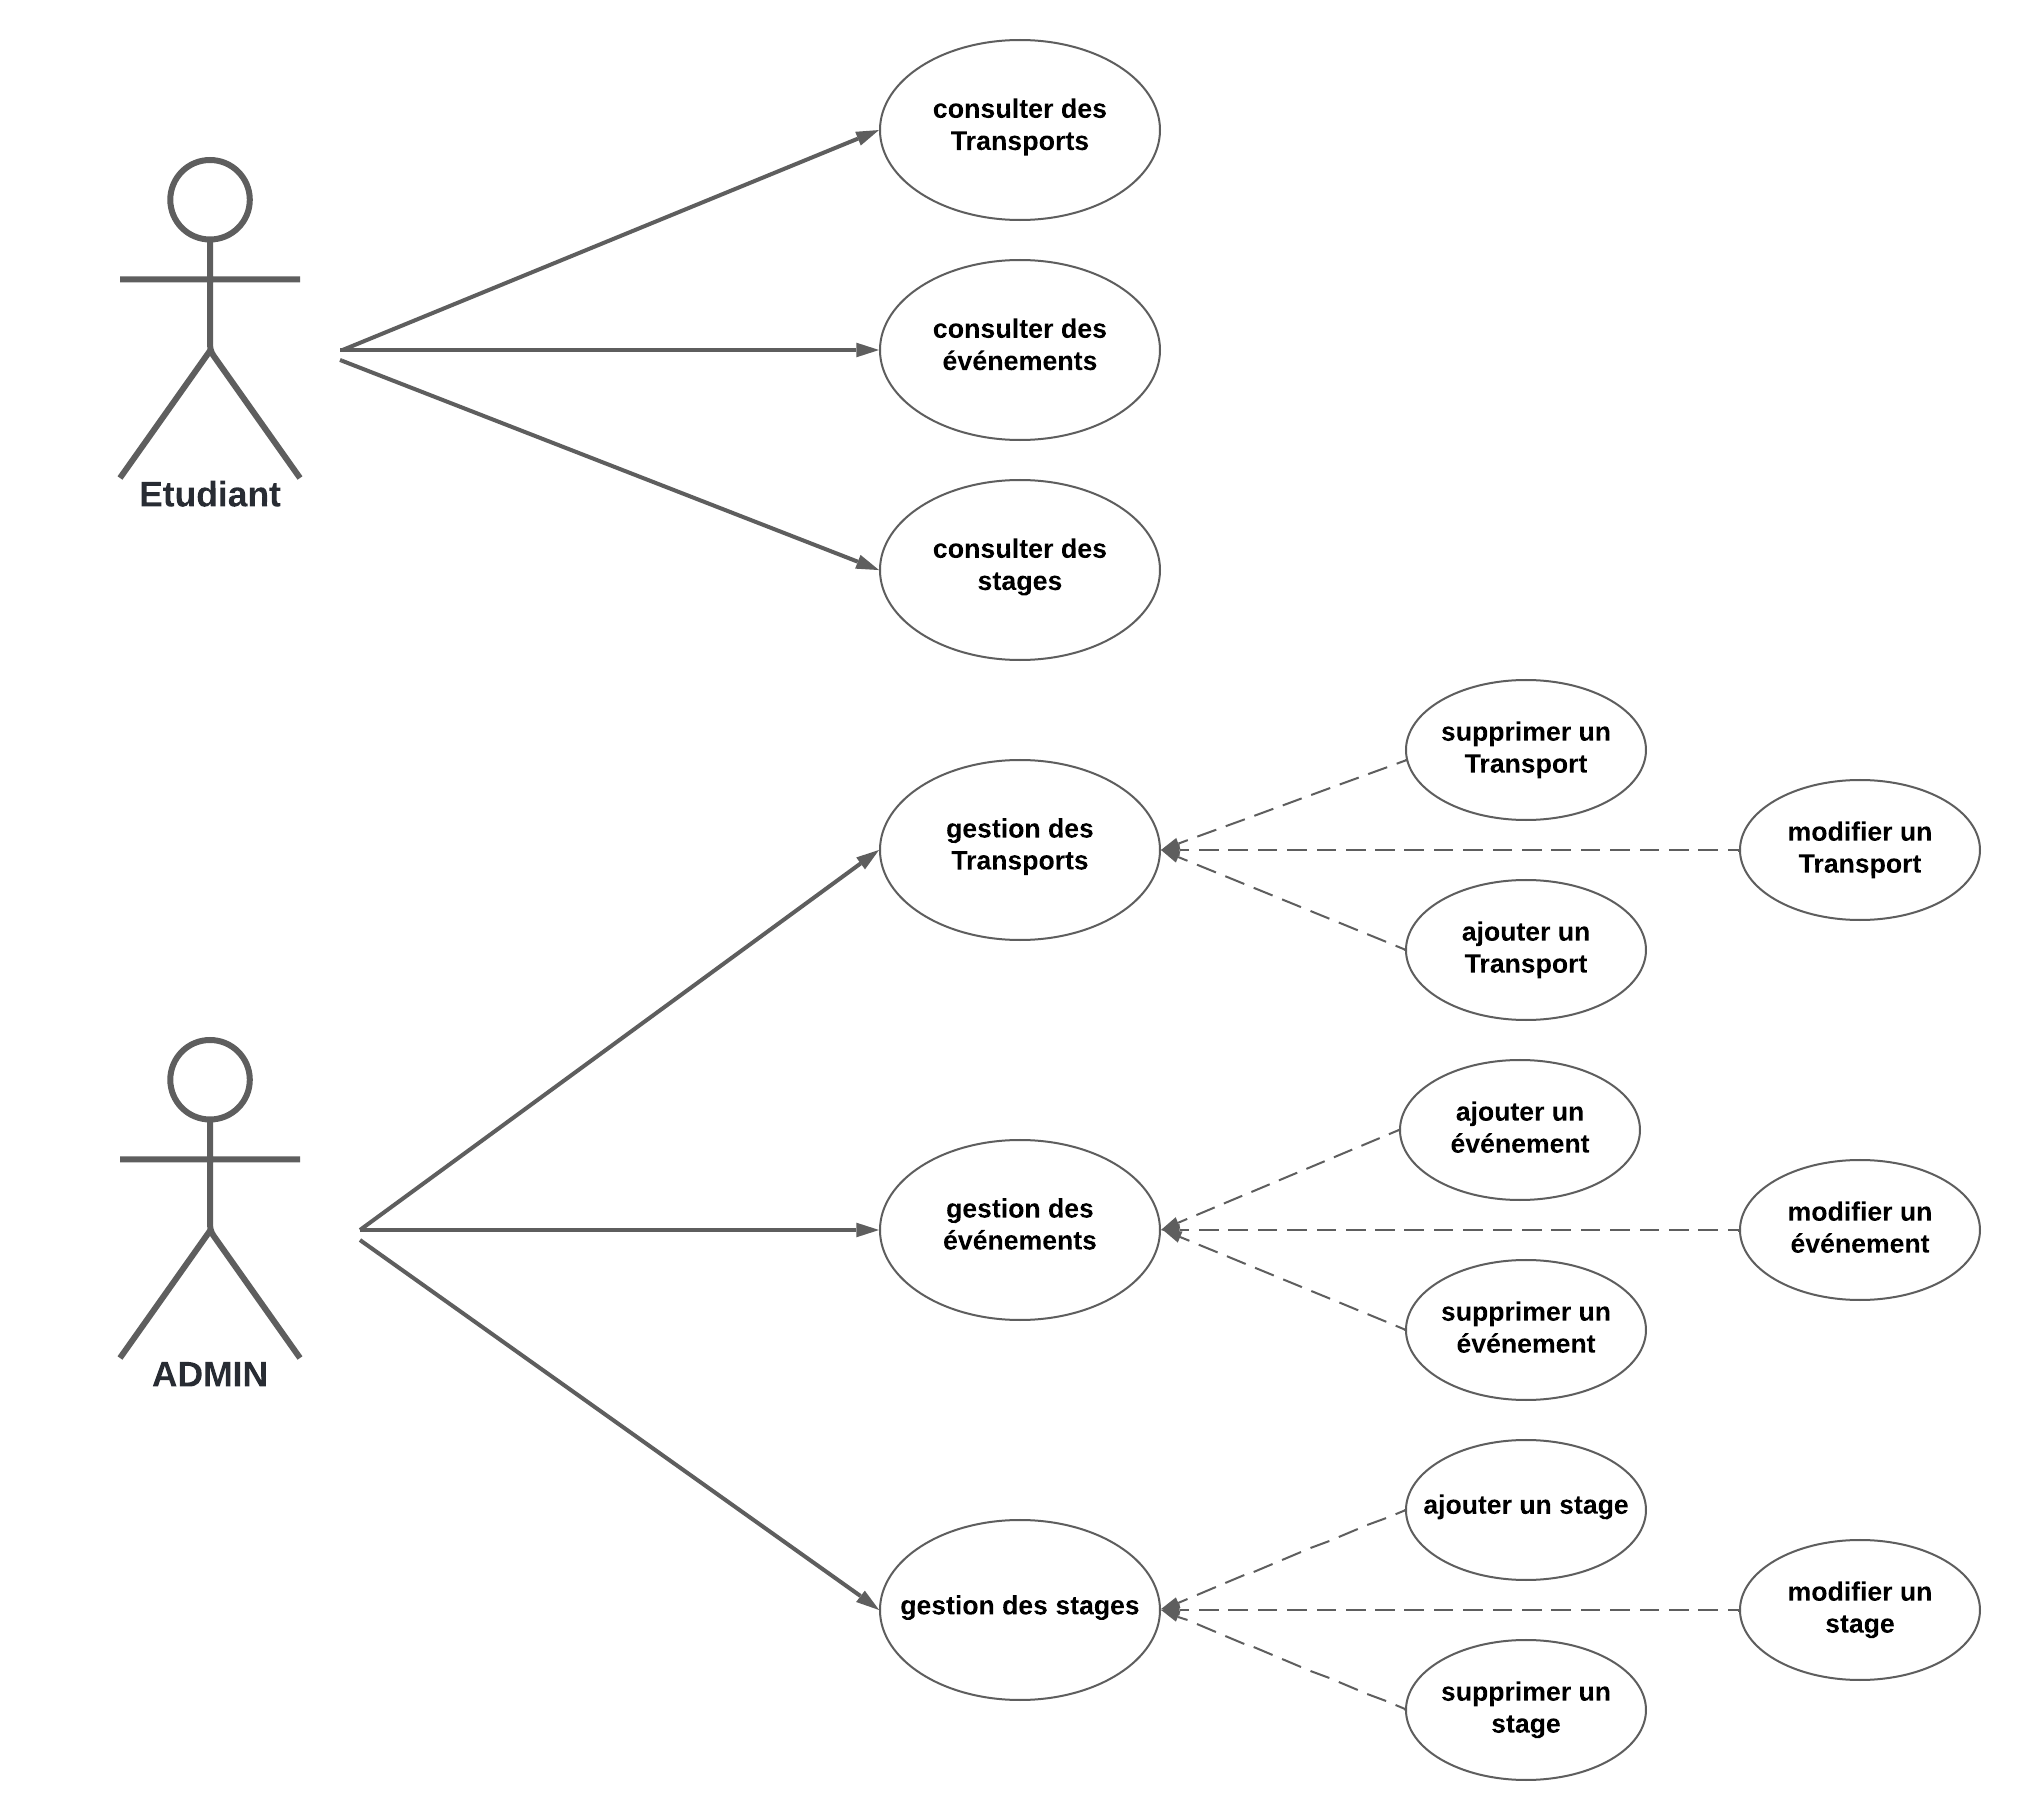
\includegraphics[height=23cm,width=15cm]{images/gestion des transport, evenements et stages.png}%
    }
    \caption{Figure du Diagramme de cas d'utilisation Sprint 3 }
\end{figure}

\subsection{Description textuelle du cas d’utilisation «Ajouter un stage»}
\vspace{-4mm}

l'admin peut saisir les détails d'un nouveau stage, vérifier les informations et les enregistrer dans le système.

\begin{table}[h]
\centering
\begin{tabular}{|p{3cm}|p{12cm}|}
\hline
\textbf{Cas d'utilisation } & Ajouter un stage \\
\hline
\textbf{Acteurs} & Admin \\
\hline
\textbf{Précondition} & Admin authentifié \\
\hline
\textbf{Postcondition} & Stage ajouté \\
\hline
\textbf{Scénario nominal} &
\begin{enumerate}
    \item L'admin est sur la page d'accueil.
    \item L'admin choisit "Stages" dans la barre latérale.
    \item L'admin clique sur le bouton "Ajouter un stage".
    \item Le système affiche le formulaire d'ajout de stage.
    \item L'admin remplit le formulaire avec les détails du stage.
    \item L'admin soumet le formulaire.
    \item Le système enregistre les informations du stage et le stage est ajouté à la liste des stages disponibles.
\end{enumerate} \\
\hline
\textbf{Exception} & Le système affiche un message d'erreur si un champ obligatoire n'est pas rempli dans le formulaire d'ajout de stage. \\
\hline 
\end{tabular}
\caption{Description du cas d’utilisation « Ajouter un stage »}
\end{table}

\vspace{-1.3cm}

\subsection{Description textuelle du cas d’utilisation «Modifier un stage»}
\vspace{-4mm}
l'admin peut saisir les détails d'un nouveau stage, vérifier les informations et les enregistrer dans le système.

\begin{table}[h]
\centering
\begin{tabular}{|p{3cm}|p{12cm}|}
\hline
\textbf{Cas d'utilisation } & Modifier un stage \\
\hline
\textbf{Acteurs} & Admin \\
\hline
\textbf{Précondition} & Admin authentifié \\
\hline
\textbf{Postcondition} & Stage modifié \\
\hline
\textbf{Scénario nominal} &
\begin{enumerate}
    \item L'admin est sur la page d'accueil.
    \item L'admin choisit "Stages" dans la barre latérale.
    \item L'admin consulte la liste des stages.
    \item L'admin sélectionne le stage à modifier.
    \item Le système affiche le formulaire de modification de stage.
    \item L'admin modifie les détails du stage.
    \item L'admin soumet le formulaire de modification.
    \item Le système enregistre les modifications et le stage est mis à jour dans la liste des stages disponibles.
\end{enumerate} \\
\hline
\textbf{Exception}& Un champ obligatoire n'est pas rempli. Le système affiche un message d'erreur si un champ obligatoire n'est pas rempli dans le formulaire de modification de stage. \\
\hline 
\end{tabular}
\caption{Description du cas d’utilisation « Modifier un stage »}
\end{table}

\newpage

\subsection{Description textuelle du cas d’utilisation «Supprimer un stage»}
\vspace{-6mm}
l'admin peut retirer un stage existant de la base de données.
\begin{table}[h]
\centering
\begin{tabular}{|p{3cm}|p{12cm}|}
\hline
\textbf{Cas d'utilisation } & Supprimer un stage \\
\hline
\textbf{Acteurs} & Admin \\
\hline
\textbf{Précondition} & Admin authentifié \\
\hline
\textbf{Postcondition} & Stage supprimé \\
\hline
\textbf{Scénario nominal} &
\begin{enumerate}
    \item L'admin est sur la page d'accueil.
    \item L'admin choisit "Stages" dans la barre latérale.
    \item L'admin consulte la liste des stages.
    \item L'admin sélectionne le stage à supprimer.
    \item Le système affiche une confirmation de suppression.
    \item L'admin confirme la suppression.
    \item Le système supprime le stage de la liste des stages disponibles.
\end{enumerate} \\
\hline
\end{tabular}
\caption{Description du cas d’utilisation « Supprimer un stage »}
\end{table}
\vspace{-1.7cm}
\section{Diagramme de séquence }
\vspace{-6mm}
Les diagrammes de séquence illustrent les interactions lors de la gestion des stages, offrant une vue claire des processus impliqués.
\vspace{-1cm}
\subsection{Diagramme de séquence «Ajouter un Stage»}
\vspace{-6mm}
Le diagramme présente le processus d'ajout d'un nouveau stage par l'admin sur la partie web de notre application.
\vspace{-4mm}
\begin{figure}[H]%
    \center%
    \setlength{\fboxsep}{5pt}%
    \setlength{\fboxrule}{0.5pt}%
    \fbox{
    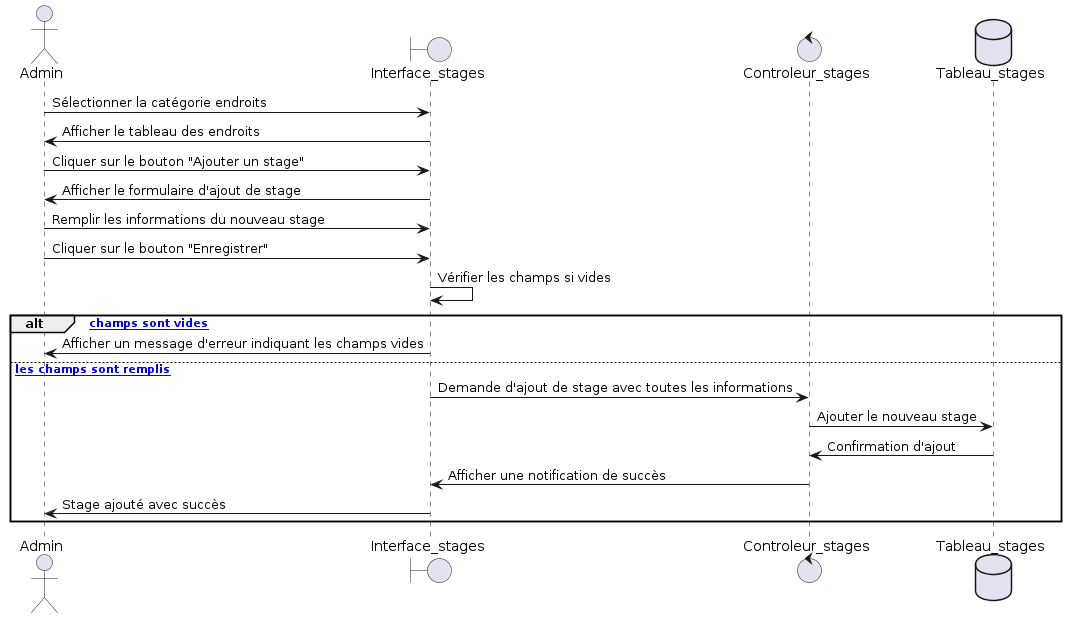
\includegraphics[height=9cm,width=15cm]{images/ffffajoutstages.png}%
    }
    \caption{Figure du Diagramme de séquence «Ajouter un stage» }
\end{figure}

\subsection{Diagramme de séquence «Modifier un Stage»}
\vspace{-6mm}
Le diagramme illustre le processus de modification d'un stage par l'admin sur la partie web de notre application.
\vspace{-4mm}
\begin{figure}[H]%
    \center%
    \setlength{\fboxsep}{5pt}%
    \setlength{\fboxrule}{0.5pt}%
    \fbox{
    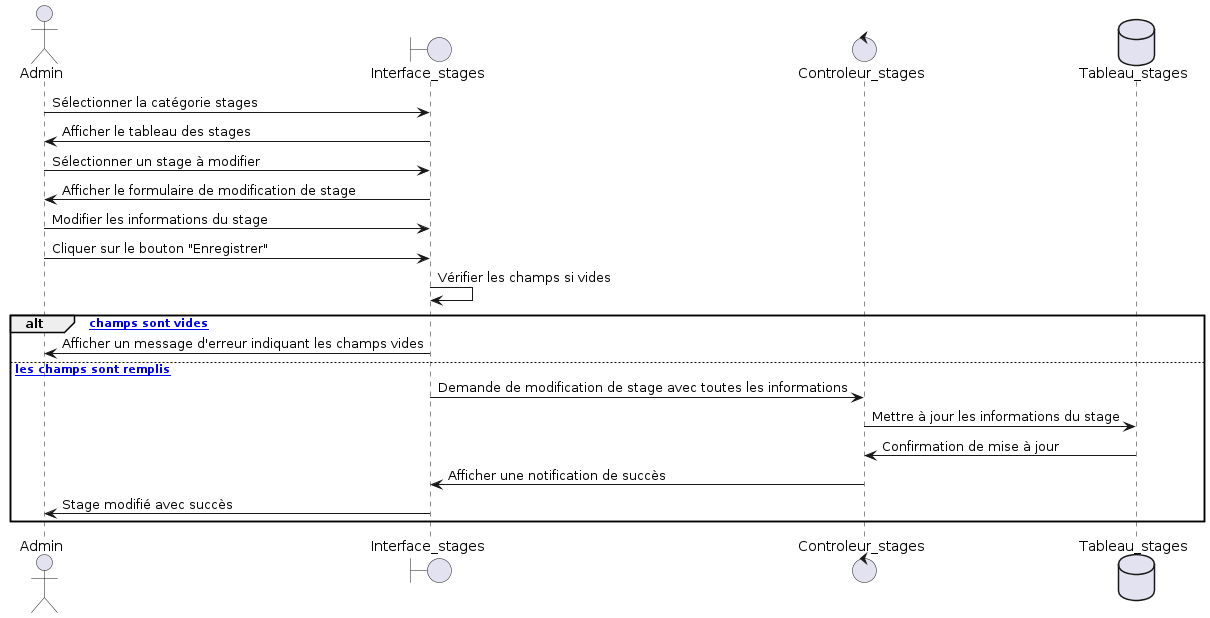
\includegraphics[height=8.5cm,width=15cm]{images/ffffeditstage.png}%
    }
    \caption{Diagramme de séquence «modifier un stage» }
\end{figure}
\vspace{-1.7cm}
\subsection{Diagramme de séquence «Supprimer un Stage»}
\vspace{-6mm}
Le diagramme décrit le processus de suppression d'un stage par l'admin sur la partie web de notre application.
\vspace{-2mm}
\begin{figure}[H]%
    \center%
    \setlength{\fboxsep}{5pt}%
    \setlength{\fboxrule}{0.5pt}%
    \fbox{
    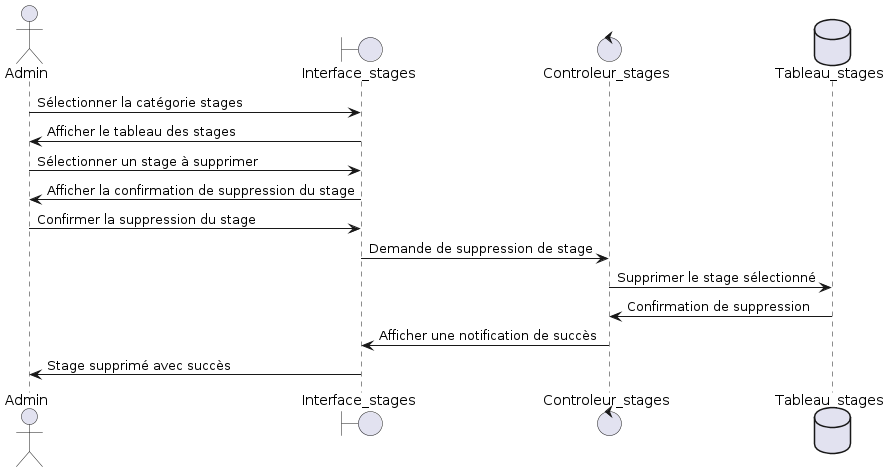
\includegraphics[height=8.5cm,width=15cm]{images/fffffsuppstage.png}%
    }
    \caption{Diagramme de séquence supprimer un stage }
\end{figure}
\vspace{-7mm}
\section{Diagramme de classes }
\vspace{-4mm}
Le diagramme de classes présenté ci-dessus illustre la structure des entités clés de notre système de gestion, à savoir les stages, les événements et les transports. Chaque entité est représentée par une classe correspondante, comprenant des attributs décrivant ses caractéristiques principales ainsi que des méthodes pour accéder et manipuler ces données. Cette conception permet une modélisation claire et cohérente des différentes fonctionnalités de notre application.

\begin{figure}[H]%
    \center%
    \setlength{\fboxsep}{5pt}%
    \setlength{\fboxrule}{0.5pt}%
    \fbox{
    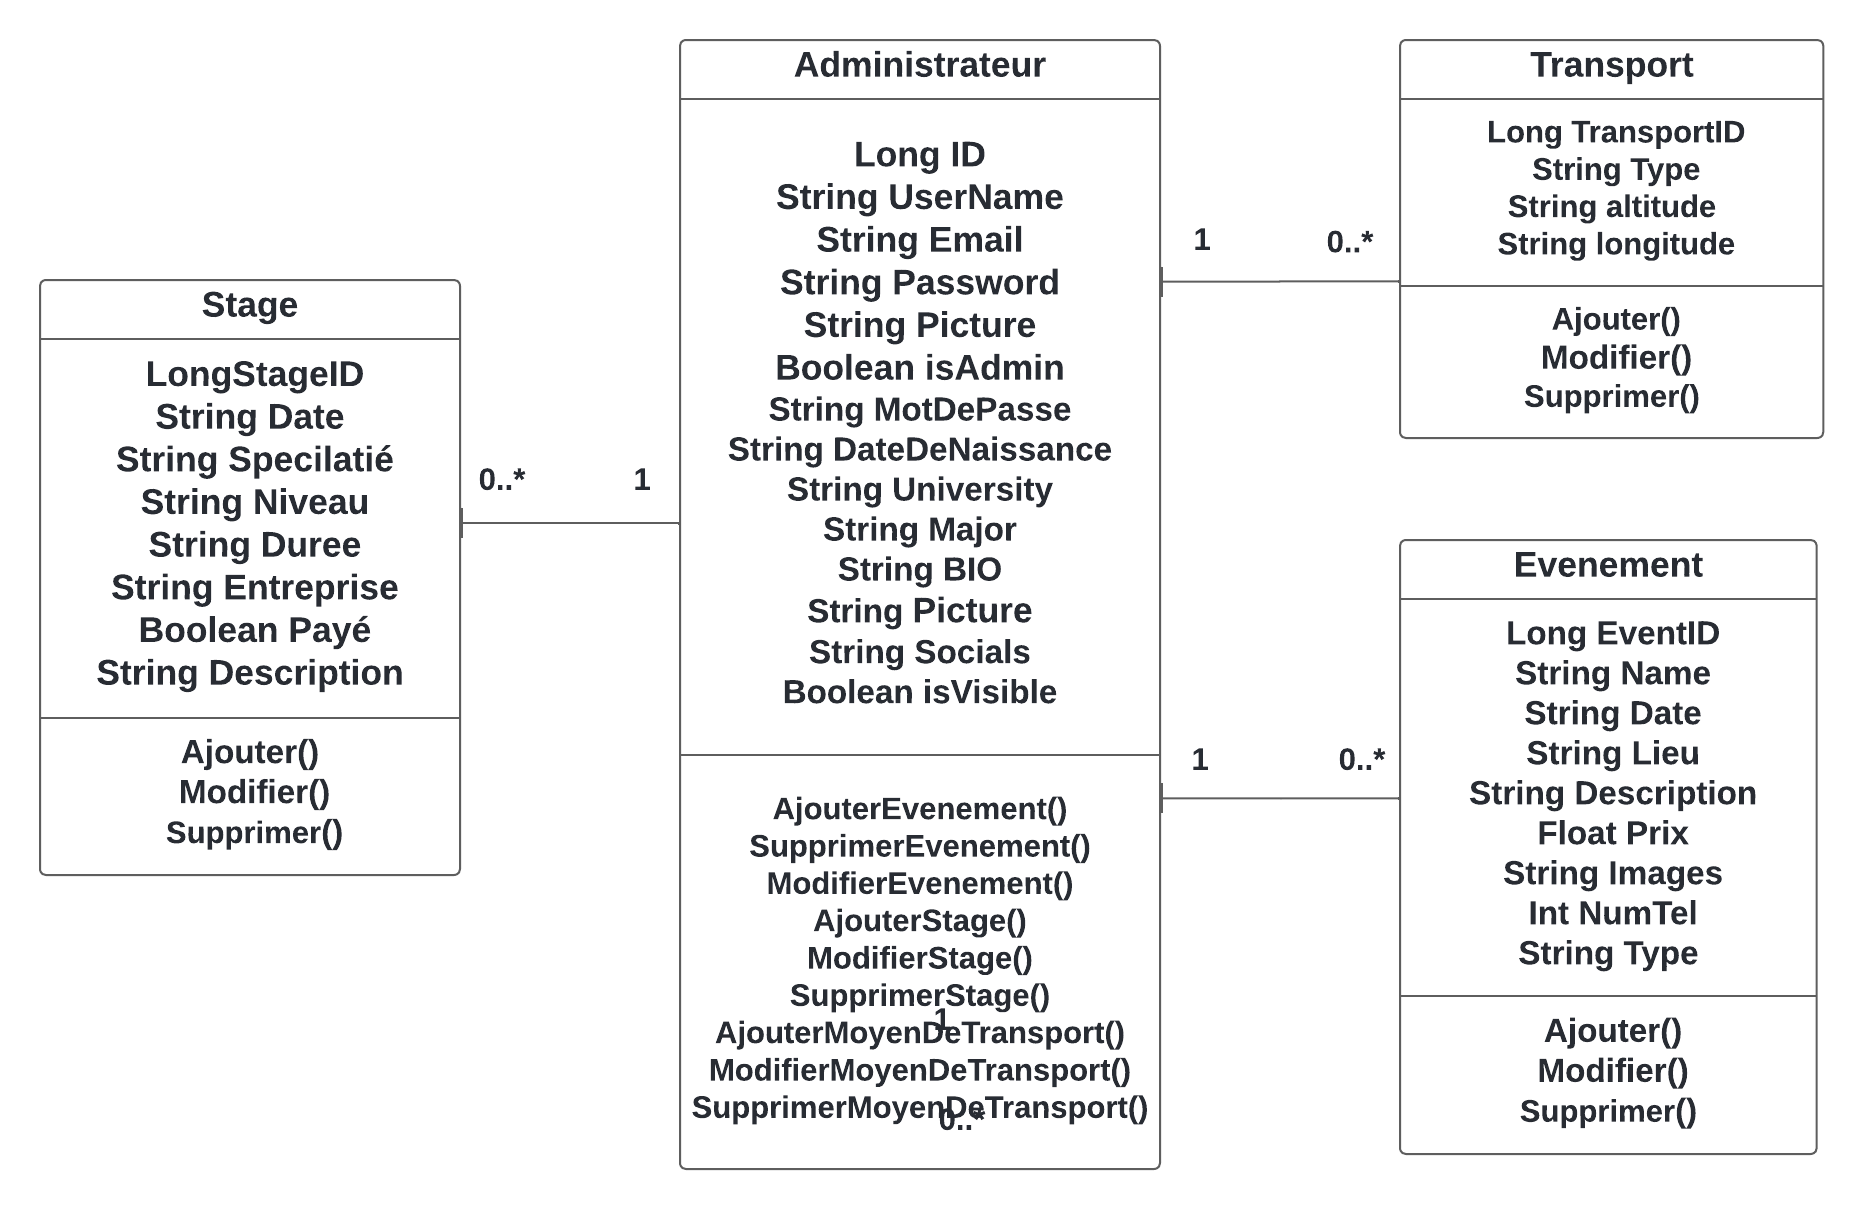
\includegraphics[height=16.5cm,width=15cm]{images/AAATransportations.png}%
    }
    \caption{Diagramme de classes Sprint 3}
\end{figure}
\vspace{-4mm}
\section{Réalisation }
\vspace{-4mm}
La partie de réalisation représente la dernière phase du cycle de développement d’un sprint. Elle permet de présenter les résultats obtenus lors de l’étape de développement afin d’assurer et de garantir une version de qualité. Nous allons montrer cela par des captures d’écrans des fonctionnalités ayant été développées.

\vspace{-9mm}
\subsection{Ajout d'un évenement}
\vspace{-4mm}
L'interface web pour l'admin permet d'ajouter des événements. Via le menu de navigation, l'admin accède à un formulaire pour entrer le titre, la description, la date, l'heure et le lieu de l'événement. Une fois soumis, l'événement est visible pour les utilisateurs de l'application mobile.

\begin{figure}[h]
    \centering
    \begin{minipage}[b]{0.45\linewidth}
        \centering
        \setlength{\fboxsep}{5pt}%
        \setlength{\fboxrule}{0.5pt}%
        \fbox{
        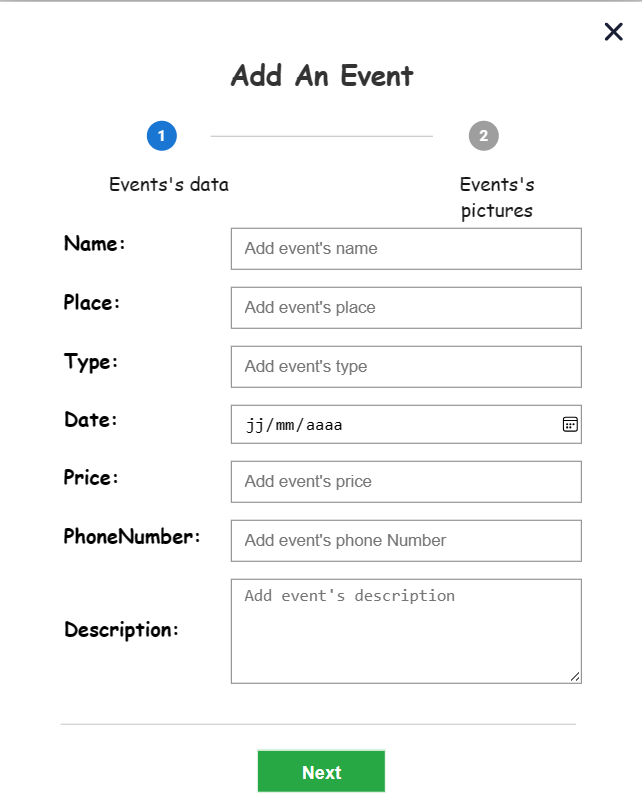
\includegraphics[height=12cm,width=8cm]{images/XAddEvent1.png}
        }
        \caption{Interface d'ajout d'un évenement}
        \label{fig:image1}
    \end{minipage}
    \hfill
    \begin{minipage}[b]{0.45\linewidth}
        \centering
        \setlength{\fboxsep}{5pt}%
        \setlength{\fboxrule}{0.5pt}%
        \fbox{
        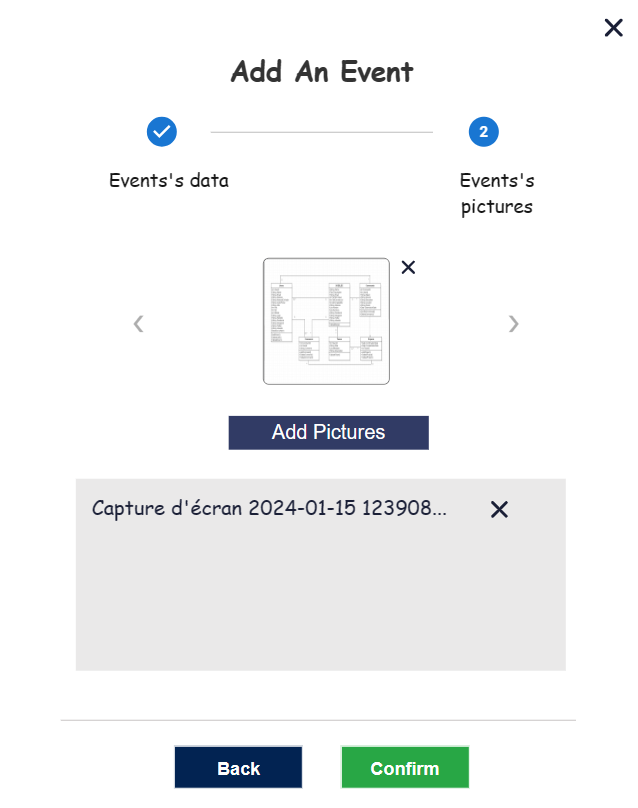
\includegraphics[height=12cm,width=8cm]{images/XAddEvent2.png}
        }
        \caption{Diagramme de classes publication et notification}
        \label{fig:image2}
    \end{minipage}
\end{figure}


\subsection{Modification d'un stage}
\vspace{-6mm}
L'admin peut modifier les détails des stages via l'interface web, incluant titre, description, durée, exigences et lieu, visibles immédiatement sur l'application mobile.
\vspace{-4mm}
\begin{figure}[H]%
    \center%
    \setlength{\fboxsep}{5pt}%
    \setlength{\fboxrule}{0.5pt}%
    \fbox{
    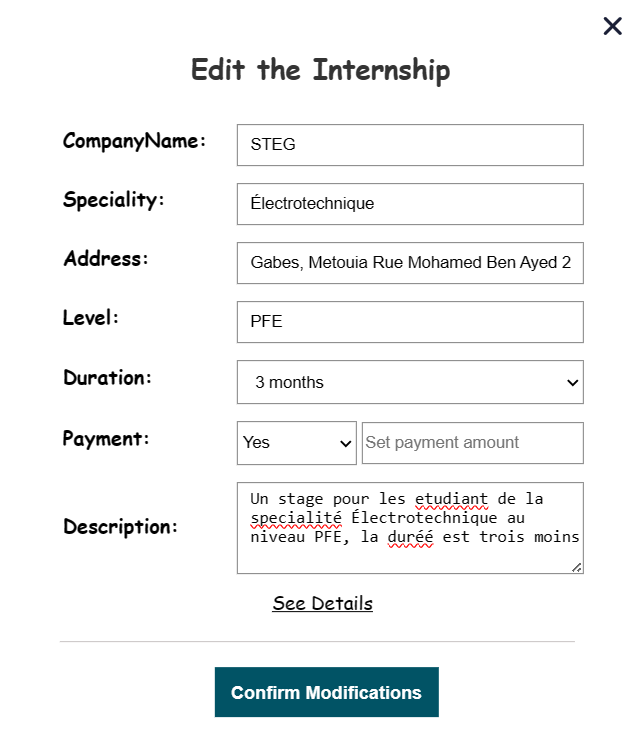
\includegraphics[height=10cm,width=10cm]{images/XEditInternship.png}%
    }
    \caption{Interface de modification d'un stage}
\end{figure}
\vspace{-1.9Cm}
\section{Effacer un moyen du transport }
\vspace{-6mm}
L'interface web admin permet de supprimer des transports en sélectionnant et confirmant leur suppression de l'application mobile.
\vspace{-4mm}
\begin{figure}[H]%
    \center%
    \setlength{\fboxsep}{5pt}%
    \setlength{\fboxrule}{0.5pt}%
    \fbox{
    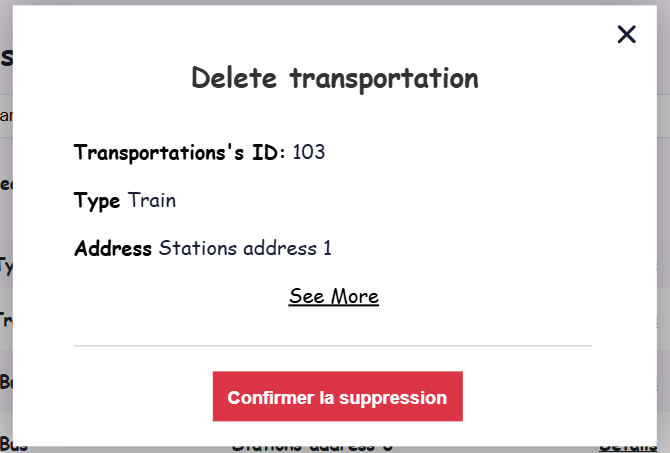
\includegraphics[height=7cm,width=13cm]{images/AAADeleteTrasportation.png}%
    }
    \caption{Interface de supression d'un stage}
\end{figure}
\vspace{-1.3cm}
\subsection{Evenement partie Mobile }
\vspace{-6mm}
Sur l'application mobile, les utilisateurs peuvent consulter les  événements, incluant le titre, la description, la date, l'heure, le lieu, ainsi que les images associées à chaque événement.
\vspace{-2mm}
\begin{figure}[H]%
    \center%
    \setlength{\fboxsep}{5pt}%
    \setlength{\fboxrule}{0.5pt}%
    \fbox{
    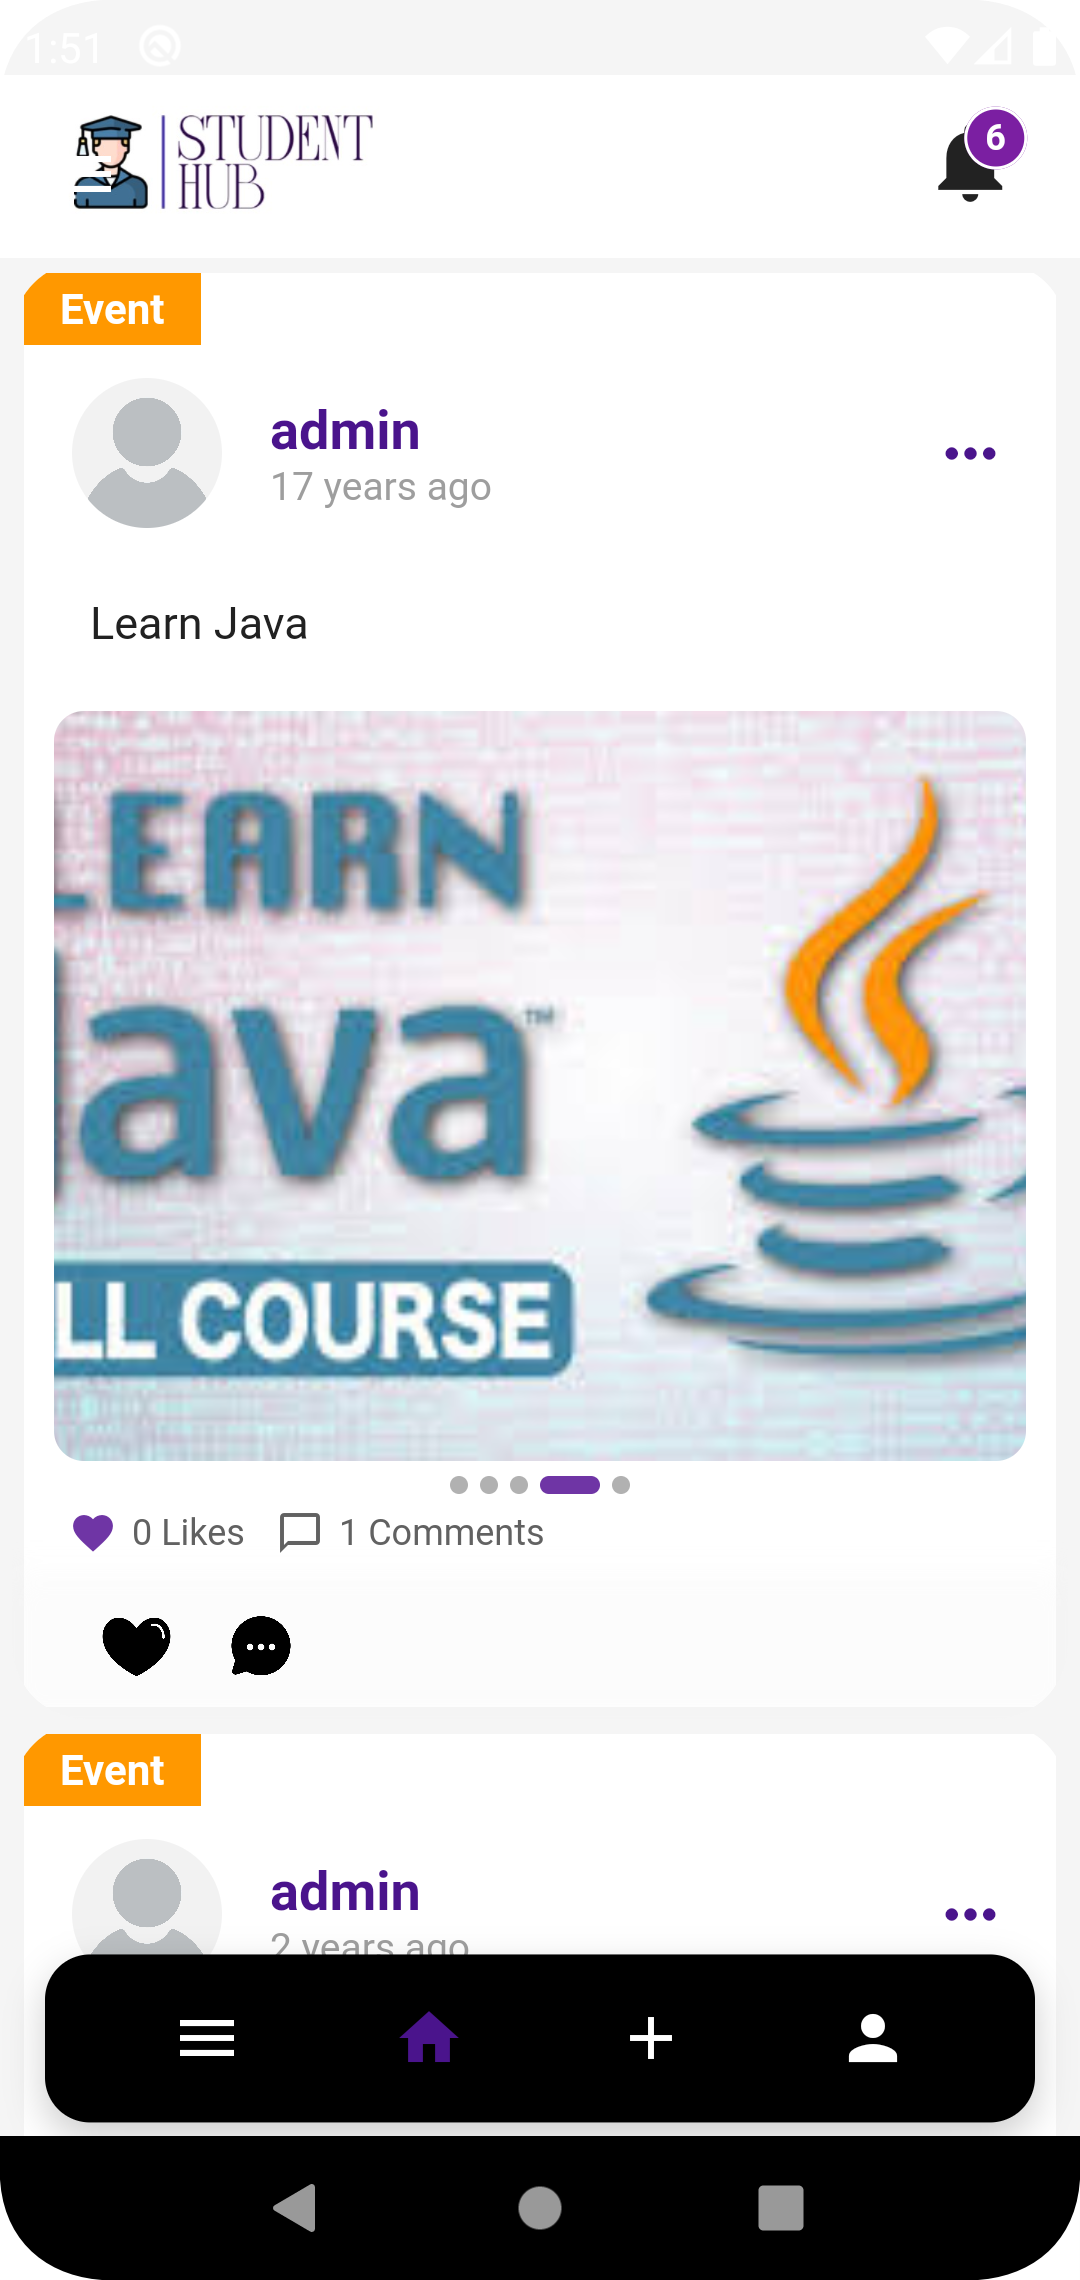
\includegraphics[height=8.7cm,width=7cm]{images/AAAEventPublication.png}%
    }
    \caption{Interface d'un évenement dans la partie mobile}
\end{figure}
\vspace{-1.8Cm}
\subsection{Stage partie mobile }
\vspace{-6mm}
Les utilisateurs peuvent voir les détails des offres de stages, y compris le titre, la description, les qualifications requises, les dates et le lieu.
\vspace{-2mm}
\begin{figure}[H]%
    \center%
    \setlength{\fboxsep}{5pt}%
    \setlength{\fboxrule}{0.5pt}%
    \fbox{
    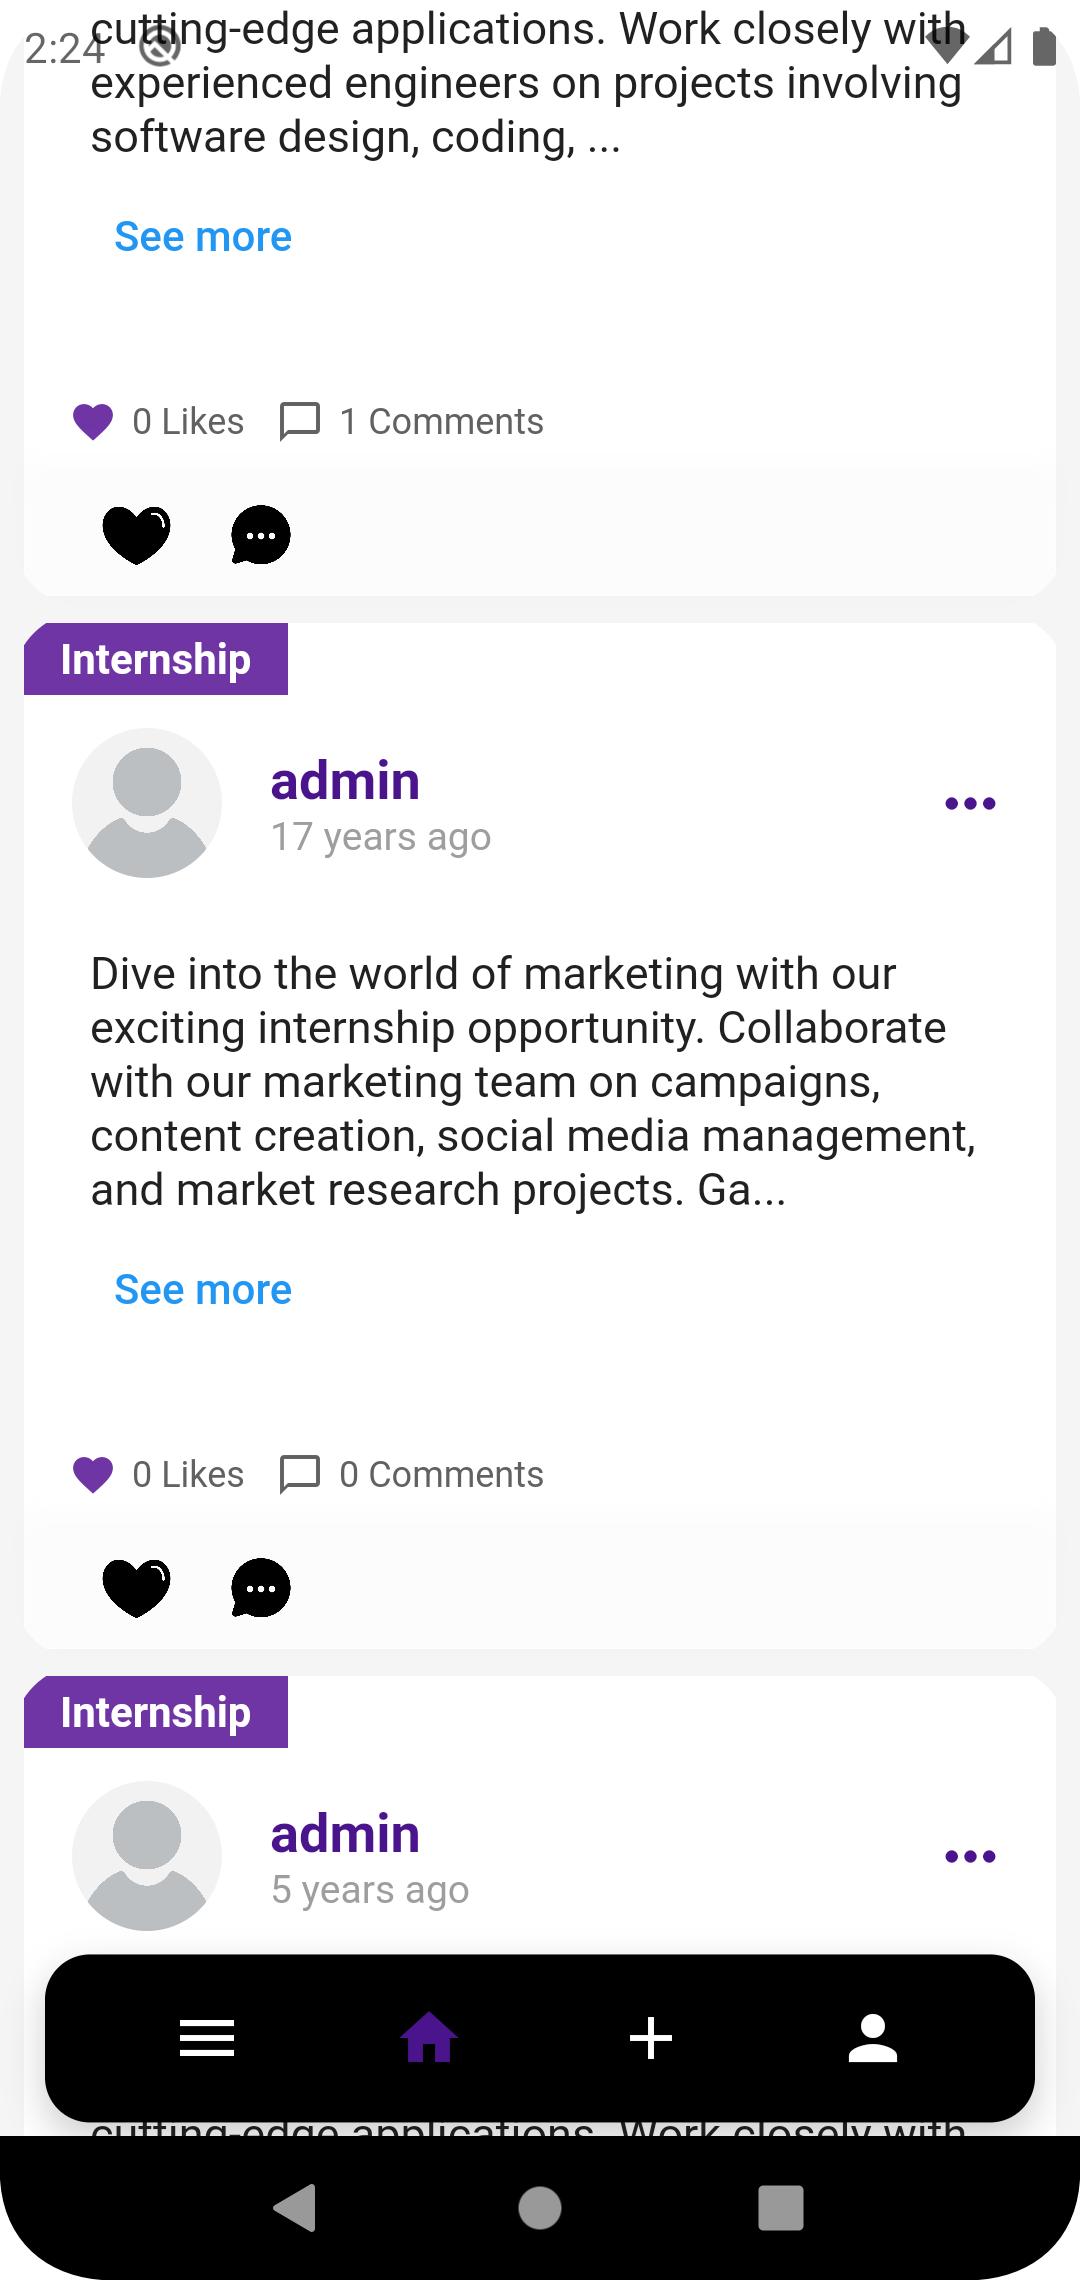
\includegraphics[height=8.7cm,width=7cm]{images/AAAInternshipPublications.png}%
    }
    \caption{Interface d'un stage dans la partie mobile}
\end{figure}
\vspace{-1cm}
\subsection{Les moyens des transports partie mobile }
\vspace{-4mm}
Sur l'application mobile, les utilisateurs peuvent consulter les informations sur les transports. Chaque entrée affiche les détails tels que le type de transport, les horaires et les itinéraires. Les utilisateurs peuvent également voir les mises à jour en temps réel sur les retards ou les changements de service.
\begin{figure}[H]%
    \center%
    \setlength{\fboxsep}{5pt}%
    \setlength{\fboxrule}{0.5pt}%
    \fbox{
    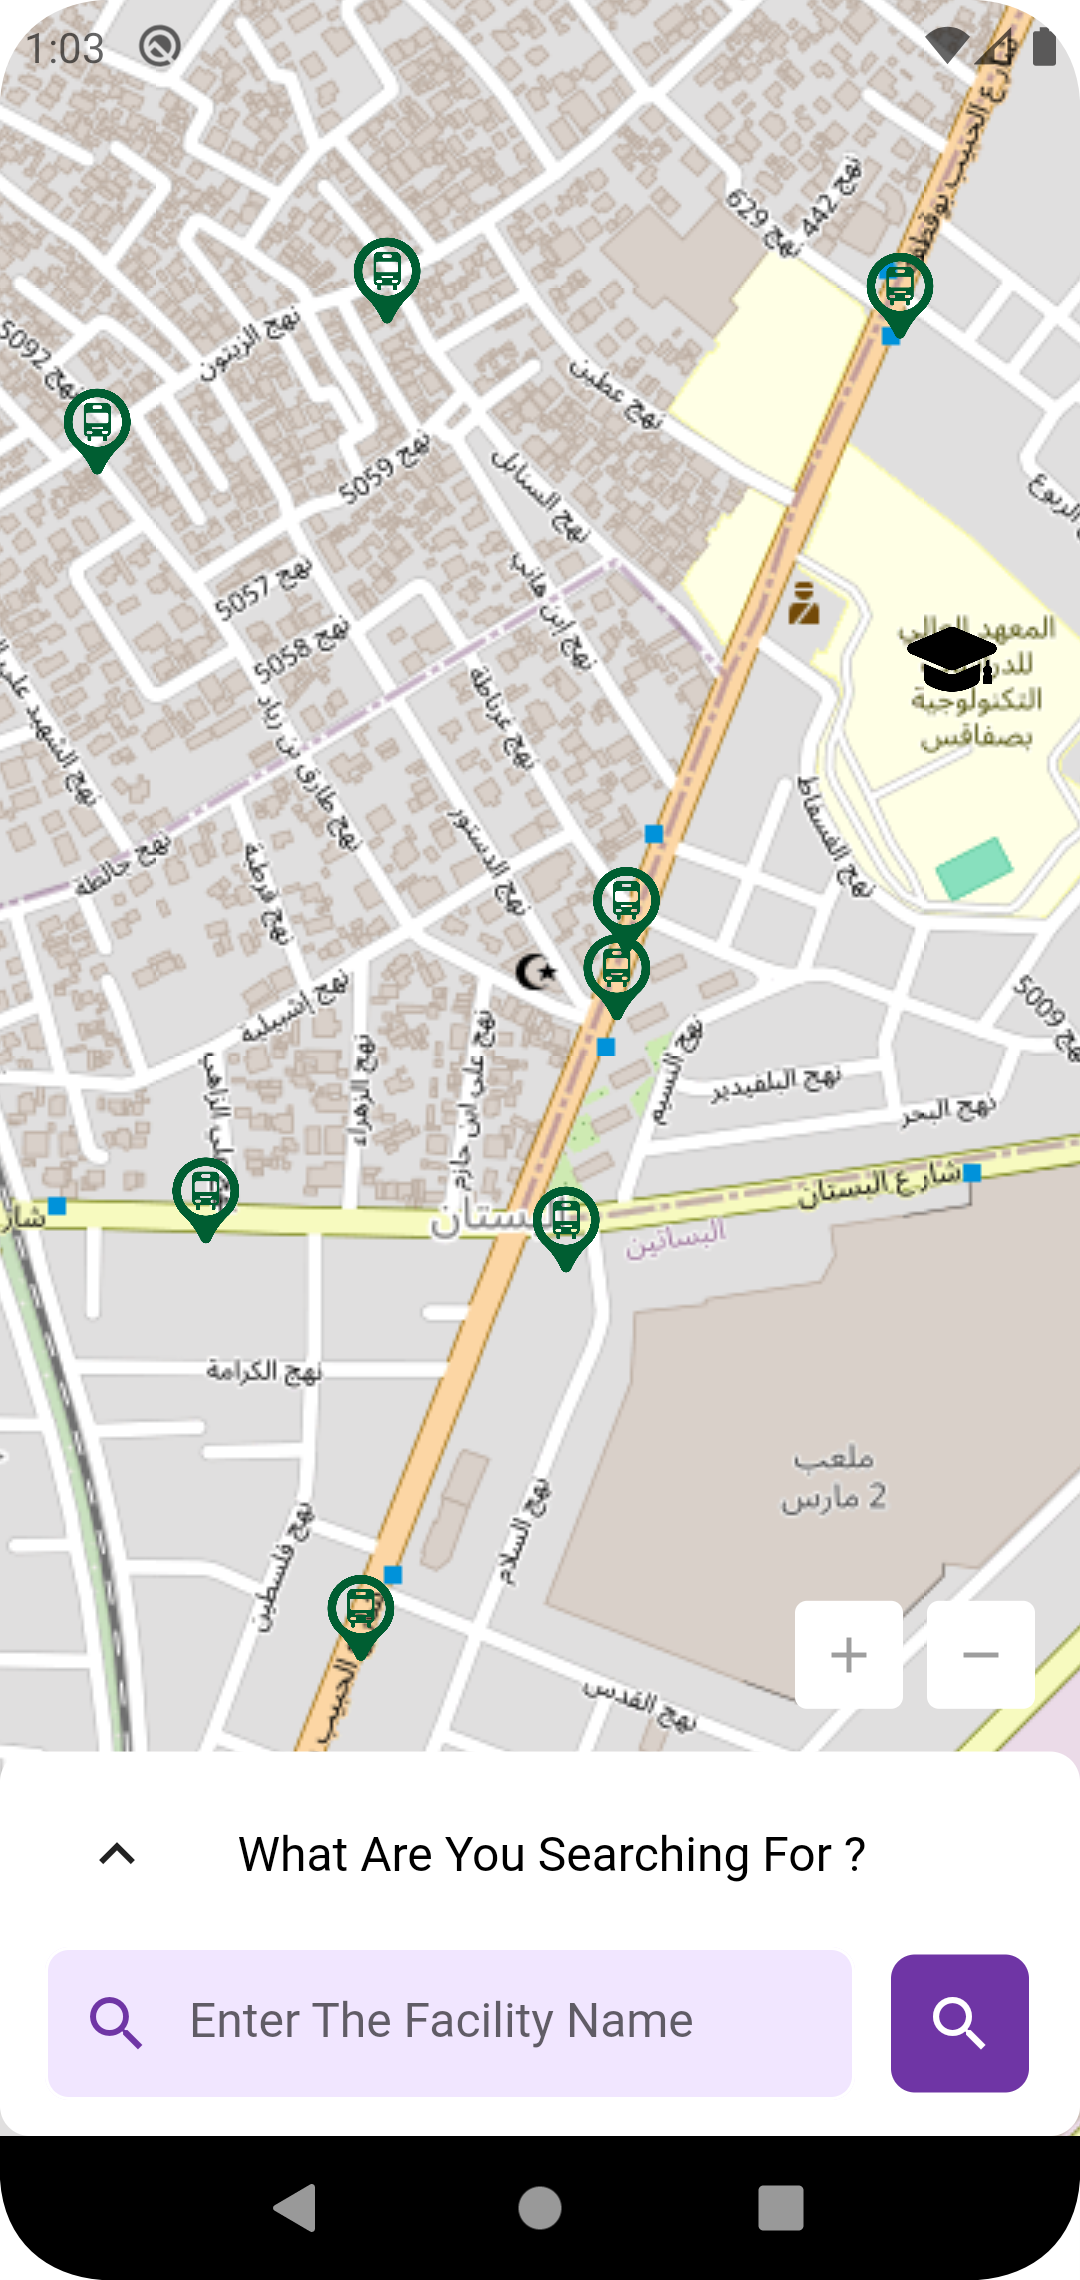
\includegraphics[height=10cm,width=7cm]{images/AAATransportStations.png}%
    }
    \caption{Interface du moyen de transport dans la partie mobile}
\end{figure}

\vspace{-1cm}

\section{Conclusion }
\vspace{-4mm}
En conclusion, ce sprint se focalise sur l'optimisation de la gestion du transport, des événements et des stages au sein de notre application. En dotant les admins d'outils performants et intuitifs, nous visons à améliorer l'affichage des moyens transports disponibles, à faciliter l'organisation et la communication autour des événements, et à simplifier l'accès aux opportunités de stage pour les utilisateurs. Ce sprint représente une étape clé pour renforcer l'efficacité administrative et offrir une expérience utilisateur enrichie et fluide.

\end{sloppypar} 
